\chapter[Организация ввода-вывода в \Sys{C++}]{Организация ввода-вывода в \Sys{C++}}
\section[Форматированный ввод-вывод в \Sys{C++}]{Форматированный ввод-вывод в \Sys{C++}}
В этом параграфе мы вернёмся к рассмотренным ранее \emph{конструкциям} \Sys{cin} и
\Sys{cout}, и рассмотрим возможности их использования для организации \emph{форматированного 
}\index{Оператор!ввода}\emph{ввода}-\index{Оператор!вывода}\emph{вывода}.


Для управления вводом-выводом в \Sys{C++} используются:

\begin{itemize}
\item \emph{флаги} форматного ввода-вывода;
\item \emph{манипуляторы} форматирования.
\end{itemize}

\subsection[Использование флагов форматного ввода-вывода]{Использование флагов форматного ввода-вывода}
\label{ch07:1.1}
\emph{Флаги} позволяют включить или выключить один из параметров вывода
на экран. Для \emph{установки флага вывода} используется следующая конструкция языка
\Sys{C++}:

\Sys{cout.setf(ios::flag)}

Для \emph{снятия флага} применяют конструкцию 

\Sys{cout.unsetf(ios::flag)}

здесь \Sys{flag} --- имя конкретного флага.

Если при выводе необходимо установить несколько флагов, то можно воспользоваться арифметической операцией «или»
(\Sys{\textbar}). В этом случае конструкция языка \Sys{C++} будет такой:

\Sys{cout.setf(ios::flag1{\textbar}ios::flag2{\textbar}ios::flag3)}

В данном случае \Sys{flag1}, \Sys{flag2}, \Sys{flag3} --- имена устанавливаемых
флагов вывода.

В таблице \ref{ch07:refTable0} приведены некоторые \emph{флаги форматного вывода} с примерами их
использования. 


{\tabcolsep=0.1em\noindent\footnotesize
\begin{longtable}{|l|p{0.28\textwidth}|p{0.37\textwidth}|p{0.2\textwidth}|}
\caption{Некоторые флаги форматного вывода} \label{ch07:refTable0}\\
\hline
\Emph{Флаг} &\Emph{Описание} &\Emph{Пример использования\footnotemark} &\Emph{Результат}\\
\hline \hline
\endfirsthead
\multicolumn{4}{c}%
{{\tablename\ \thetable{} --- продолжение}} \\
\hline
\Emph{Флаг} &\Emph{Описание} &\Emph{Пример использования} &\Emph{Результат}\\
\hline \hline
\endhead
\Sys{right} &\raggedright Выравнивание по правой границе &
\lstinline!int r=-25;!\linebreak
\lstinline!cout.setf(ios::right);!\linebreak
\lstinline!cout.width(15);!\linebreak
\lstinline!cout<<"r="<<r<<endl;!
&\ \linebreak\ \linebreak\ \linebreak\Sys{r=-25}\\\hline
\Sys{left}&\raggedright Выравнивание по левой границе (по умолчанию)&
\lstinline!double r=-25.45;!\linebreak
\lstinline!cout.setf(ios::left);!\linebreak
\lstinline!cout.width(50);!\linebreak
\lstinline!cout<<"r="<<r<<endl;!
&\ \linebreak\ \linebreak\ \linebreak\Sys{r=-25.45}\\\hline
\Sys{boolalpha} &\raggedright Вывод логических величин в текстовом виде (\Sys{true}, \Sys{false}) &
\lstinline!bool a=true;!\linebreak
\lstinline!cout<<a<<endl;!\linebreak
\lstinline!cout.setf(ios::boolalpha);!\linebreak
\lstinline!cout<<a<<endl;!
&\ \linebreak 1\linebreak\ \linebreak true\\\hline
\Sys{dec} &\raggedright Вывод величин в десятичной системе счисления (по умолчанию) &
\lstinline!int r=-25;!\linebreak 
\lstinline!cout<<"r="<<r<<endl;!
&\ \linebreak\Sys{r=-25}\\\hline
\Sys{oct} &\raggedright Вывод величин в восьмеричной системе счисления&% (для этого надо снять флаг вывод в десятичной) &
\lstinline!int p=23;!\linebreak
//\emph{\Sys{Отменить, установленный по умолчанию, вывод в десятичной системе счисления}}\linebreak
\lstinline!cout.unsetf(ios::dec);!\linebreak
//\emph{\Sys{Установить вывод в восьмеричной системе счисления}}\linebreak
\lstinline!cout.setf(ios::oct);!\linebreak
\lstinline!cout<<"p="<<p<<endl;!
&
\ \linebreak\ \linebreak\ \linebreak \linebreak\linebreak\linebreak\linebreak\linebreak \Sys{p=27}\\\hline
\Sys{hex} &\raggedright Вывод величин в шестнадцатеричной системе счисления&% (для этого надо снять флаг вывод в десятичной) &
\lstinline!int p=23;! \linebreak
//\emph{\Sys{Отменить, установленный по умолчанию, вывод в десятичной системе счисления}}\linebreak
\lstinline!cout.unsetf(ios::dec);!\linebreak
//\emph{\Sys{Установить вывод в шестнадцатеричной системе счисления}}\linebreak
\lstinline!cout.setf(ios::hex);!\linebreak 
\lstinline!cout<<"p="<<p<<endl;!
&\ \linebreak\ \linebreak\ \linebreak\linebreak\linebreak\linebreak\linebreak\linebreak\linebreak\Sys{p=17}\\\hline
\Sys{showbase} &\raggedright Выводить индикатор основания системы счисления &
\lstinline!int p=23;!\linebreak
\lstinline!cout.unsetf(ios::dec);!\linebreak
\lstinline!cout.setf(ios::hex| ios::showbase);!\linebreak
\lstinline!cout<<"p="<<p<<endl;!&\ \linebreak\ \linebreak\ \linebreak\ \linebreak\Sys{p=0x17}\\\hline
\Sys{uppercase} &\raggedright Использовать прописные буквы в шестнадцатеричных цифрах &
\lstinline!int p=29;!\linebreak
\lstinline!cout.unsetf(ios::dec);!\linebreak
\lstinline!cout.setf(ios::hex| ios::uppercase);!\linebreak
\lstinline!cout<<"p="<<p<<endl;!&\ \linebreak\ \linebreak\ \linebreak\ \linebreak\Sys{p=1D}\\\hline
\Sys{showpos} &\raggedright Выводить знак «$+$» для положительных чисел &
\lstinline!int p=29;!\linebreak
\lstinline!cout.setf(ios::showpos);!\linebreak
\lstinline!cout<<"p="<<p<<endl;!&\ \linebreak\ \linebreak\Sys{p=+29}\\\hline
\Sys{scientific} &\raggedright Экспоненциальная форма вывода вещественных чисел &
\lstinline!double p=146.673;!\linebreak
\lstinline!cout.setf(ios::scientific);!\linebreak
\lstinline!cout<<"p="<<p<<endl;!&\ \linebreak\ \linebreak\Sys{p=1.466730e+002}\\\hline
\Sys{fixed} &\raggedright Фиксированная форма вывода вещественных чисел (по умолчанию) &
\lstinline!double p=146.673;!\linebreak
\lstinline!cout.setf(ios::fixed);!\linebreak
\lstinline!cout<<"p="<<p<<endl;!&\ \linebreak\ \linebreak\Sys{p=146.673}\\\hline
\end{longtable}
}
\footnotetext{\Sys{cout.width(n)} устанавливает ширину поля вывода, подробнее об этом в п.~\ref{ch07:1.2}}

Флаги удобно использовать в тех случаях, когда следует изменить параметры всех последующих операторов ввода-вывода.
Использование большого количества флагов для управления одним или несколькими операторами ввода-вывода не совсем
удобно, потом все установленные флаги придётся отключать.

Ещё одним способом форматирования является использование манипуляторов непосредственно в конструкциях
\Sys{cin} и \Sys{cout}.

\subsection[Использование манипуляторов форматирования]{Использование манипуляторов форматирования}
\label{ch07:1.2}

\index{Манипулятор}\emph{Манипуляторы} встраиваются непосредственно в операторы
ввода-вывода. C одним из манипуляторов (\Sys{endl}\index{Манипулятор!endl}) читатель уже встречался 
начиная с первой главы книги.
В таблице \ref{ch07:refTable1} приведены основные манипуляторы форматирования с примерами их использования. Для
корректного использования всех манипуляторов необходимо подключить библиотеку:

\Sys{\#include <iomanip>}

{\tabcolsep=0.1em\noindent\footnotesize
\begin{longtable}{|l|p{0.23\textwidth}|p{0.35\textwidth}|p{0.2\textwidth}|}
\caption{Некоторые манипуляторы форматирования} \label{ch07:refTable1}\\
\hline
\Emph{Манипулятор} &\Emph{Описание} &\Emph{Пример использования} &\Emph{Результат}\\
\hline \hline
\endfirsthead
\multicolumn{4}{c}%
{{\tablename\ \thetable{} --- продолжение}} \\
\hline
\Emph{Манипулятор} &\Emph{Описание} &\Emph{Пример использования} &\Emph{Результат}\\
\hline \hline
\endhead
\Sys{setw(n)} &\raggedright Определяет ширину поля вывода в $n$ символов &
\lstinline!int r=253;!\linebreak
\lstinline!cout.setf(ios::fixed);!\linebreak
\lstinline!cout<<"r="<<setw(8)<<r<<endl;!
&\ \linebreak\ \linebreak\Sys{r=\ \ \ \ \ 253}\\\hline
\Sys{setprecision(n)} &\raggedright Определяет количество цифр ($n-1$) в дробной части числа &
\lstinline!double h=1234.6578;!\linebreak
\lstinline!cout.setf(ios::fixed);!\linebreak
\lstinline!cout<<"h="<<setw(15);!\linebreak
\lstinline!cout<<setprecision(3);!\linebreak
\lstinline!cout<<h<<endl;!&\ \linebreak\ \linebreak\ \linebreak\ \linebreak\Sys{h=1234.658}\\\hline
\Sys{dec} &\raggedright Перевод числа в десятичную систему (по умолчанию) &
\lstinline!int r=0253;!\linebreak
\lstinline!cout<<"r="<<dec<<r<<endl;!&\ \linebreak\Sys{r=171}\\\hline
\Sys{oct} &\raggedright Перевод числа в восьмеричную систему  &
\lstinline!int r=253;!\linebreak
\lstinline!cout<<"r="<<oct<<r<<endl;!&\ \linebreak\Sys{r=375}\\\hline
\Sys{hex} &%\raggedright 
Перевод числа в шестнадцатеричную систему &
\lstinline!int r=253;!\linebreak
\lstinline!cout<<"r="<<hex<<r<<endl!&\ \linebreak\Sys{p=fd}\\\hline
\Sys{right} &\raggedright Выравнивание по правой границе &
\lstinline!int r=-25;!\linebreak
\lstinline!cout.width(15);!\linebreak
\lstinline!cout<<"r="<<setw(15)<<right;!\linebreak
\lstinline!cout<<r<<endl;! &\ \linebreak\ \linebreak\ \linebreak\Sys{r=-25}\\\hline
\Sys{left} &\raggedright Выравнивание по левой границе (по умолчанию) &
\lstinline!int r=-25;!\linebreak
\lstinline!cout.width(15);!\linebreak
\lstinline!cout<<"r="<<setw(15)<<left;!\linebreak
\lstinline!cout<<r<<endl;!\footnotemark&\ \linebreak\ \linebreak\ \linebreak\Sys{r=-25}\\\hline
\Sys{boolalpha} &\raggedright Вывод логических величин в текстовом виде (\Sys{true}, \Sys{false}) &
\lstinline!bool a=true;!\linebreak
\lstinline!cout<<boolalpha<<a<<endl;!&\ \linebreak\Sys{true}\\\hline
\Sys{noboolalpha} &%\raggedright 
Вывод логических величин в чис\-ло\-вом виде (1, 0) &
\lstinline!bool a=true;!\linebreak
\lstinline!cout<<noboolalpha<<a<<endl;! &\ \linebreak 1\\\hline
\Sys{showpos} &%\raggedright 
Выводить знак «$+$» для по\-ло\-жи\-тель\-ных чисел &
\lstinline!int p=29;!\linebreak
\lstinline!cout<<"p="<<showpos<<p<<endl;!&\ \linebreak\Sys{p=+29}\\\hline
\Sys{noshowpos} &%\raggedright 
Не выводить знак «$+$» для положи\-тельных чисел &
\lstinline!int p=29;!\linebreak
\lstinline!cout<<"p="<<noshowpos<<p<<endl;!\linebreak
%\lstinline!cout<<p<<endl;! 
&\ \linebreak\ \linebreak\Sys{p=29}\\\hline
\Sys{uppercase} &%\raggedright 
Использовать прописные буквы в шестнадцатеричных цифрах &
\lstinline!int p=253;!\linebreak
\lstinline!cout<<"p="<<hex<<uppercase<<p<<endl;!\linebreak
%\lstinline!cout<<p<<endl;! 
&\ \linebreak\ \linebreak\Sys{p=FD}\\\hline
\Sys{nouppercase} &%\raggedright 
Использовать строчные буквы в шестнадцатеричных цифрах &
\lstinline!int p=253;!\linebreak
\lstinline!cout<<"p="<<hex<<nouppercase;!\linebreak
\lstinline!cout<<p<<endl;! &\ \linebreak\ \linebreak\Sys{p=fd}\\\hline
\Sys{showbase} &%\raggedright 
Выводить индикатор основания системы счисления &
\lstinline!int p=253;!\linebreak
\lstinline!cout<<"p="<<hex<<uppercase<<showbase<<p<<endl;! &\ \linebreak\ \linebreak\Sys{p=0XFD}\\\hline
\Sys{noshowbase} &%\raggedright 
Не выводить индикатор основания системы счисления &
\lstinline!int p=253;!\linebreak
\lstinline!cout<<"p="<<hex<<uppercase;!\linebreak
\lstinline!cout<<noshowbase<<p<<endl;!
&\ \linebreak\ \linebreak\Sys{p=FD}\\\hline
\Sys{setfill(c)} &\raggedright Установить символ \Sys{с} как заполнитель &
\lstinline!cout<<"x="<<right<<setw(10)<<setprecision(4);!\linebreak
\lstinline|cout<<setfill('!');|\linebreak
\lstinline!cout<<(float)1/7<<endl;!\linebreak
\lstinline!cout<<"x="<<left<<setw(10);!\linebreak
\lstinline!cout<<setprecision(4);!\linebreak
\lstinline|cout<<setfill('!');|\linebreak
\mbox{\lstinline!cout<<(float)1/7<<endl;!}&\ \linebreak\ \linebreak\ \linebreak\Sys{x=!!!!0.1429}\ \linebreak\ \linebreak\ \linebreak\ \linebreak\Sys{x=0.1429!!!!}\\\hline
\Sys{scientific} &%\raggedright 
Экспоненциальная форма вывода вещественных чисел &
\lstinline!double p=146.673;!\linebreak
\lstinline!cout<<"p="<<scientific<<p<<endl;!%\linebreak
%\lstinline!cout<<p<<endl;!
&\ \linebreak\ \linebreak\Sys{p=1.466730e+002}\\\hline
\Sys{fixed} &\raggedright Фиксированная форма вывода вещественных чисел (по умолчанию) &
\lstinline!cout<<"p="<<fixed<<p<<endl;!&\Sys{p=146.673}\\\hline
\end{longtable}
}
\footnotetext{Ещё один пример приведён при использовании манипулятора \Sys{setfill}}
Кроме того, управлять шириной поля вывода можно с помощью операторов:

\begin{itemize}
\item \Sys{cout.width(n)} --- устанавливает ширину поля вывода --- $n$ позиций;
\item \Sys{cout.precision(m)} --- определяет $m$ цифр в дробной части числа.
\end{itemize}
В п.~\ref{ch07:1.1}  и ~\ref{ch07:1.2}  были рассмотрены основные возможности форматированного ввода-вывода. 
При использовании конструкций
\Sys{cin} и \Sys{cout} фактически происходит ввод-вывод в \emph{текстовый файл}.
При вводе текстовым файлом является клавиатура ПК, при выводе в качестве текстового файла выступает экран дисплея,
\Sys{cin} и \Sys{cout} фактически являются именами
\emph{потоков}\footnote{Подробнее о текстовых потоках речь пойдёт в п.~\ref{ch07:2}}, которые отвечают за ввод и
вывод в текстовый файл. Поэтому многие рассмотренные возможности форматированного ввода-вывода будут использоваться и
при обработке текстовых файлов.

Существует два основных типа файлов: \emph{текстовые} и \emph{двоичные}. Файлы позволяют
пользователю считывать большие объёмы данных непосредственно с диска, не вводя их с клавиатуры.

\section[Работа с текстовыми файлами в \Sys{C++}]{Работа с текстовыми файлами в \Sys{C++}}\label{ch07:2}
\index{Файл!текстовый}\emph{Текстовыми} называют файлы, состоящие из любых символов. Они организуются по
строкам, каждая из которых заканчивается символом «конец строки». Конец самого файла обозначается символом «конец
файла». При записи информации в текстовый файл, просмотреть который можно с помощью любого текстового редактора, все
данные преобразуются к символьному типу и хранятся в символьном виде.

Для работы с файлами используются специальные типы данных, называемые
\index{Потоки}\emph{потоками}\footnote{Вообще говоря, потоки являются классами, которым будет посвящена
специальная глава.}. Поток \Sys{ifstream} служит для работы с файлами в режиме чтения. Поток
\Sys{ofstream} служит для работы с файлами в режиме записи. Для работы с файлами в режиме как чтения, так
и записи служит поток \Sys{iofstream}.

В программах на \Sys{C++} при работе с текстовыми файлами необходимо подключать библиотеки \Sys{iostream} и
\Sys{fstream}.

Для того, чтобы \index{Файл!запись}\emph{записать данные в текстовый файл}, необходимо:
\begin{enumerate}
\item Описать переменную типа \Sys{ofstream}.
\item Открыть файл с помощью функции \Sys{open}.
\item Вывести информацию в файл.
\item Закрыть файл.
\end{enumerate}

Для того, чтобы \index{Файл!чтение}\emph{считать данные из текстового файла}, необходимо:
\begin{enumerate}
\item Описать переменную типа \Sys{ifstream}.
\item Открыть файл с помощью функции \Sys{open}.
\item Считать информацию из файла, при считывании каждой порции данных необходимо проверять достигнут ли конец файла.
\item Закрыть файл.
\end{enumerate}

\subsection[Запись информации в текстовый файл]{Запись информации в текстовый файл}
Для того, чтобы начать работать с текстовым файлом, необходимо описать переменную типа \Sys{ofstream}.
Например, с помощью оператора

\Sys{ofstream F};\footnote{Далее термин <<поток>> будет использоваться для указания переменной,
описанной как \Sys{ofstream}, \Sys{ifstream}, \Sys{iofstream}, а термин <<файл>> для указания реального файла на диске.}

будет \emph{создана переменная} \Sys{F} для \index{Файл!запись}\emph{записи
информации в файл}. На следующем этапе файл необходимо
\index{Файл!открыть}\emph{открыть для записи}. В общем случае оператор открытия потока
будет иметь вид:

\lstinline!F.open("file", mode);!

Здесь \Sys{F} --- переменная, описанная как \Sys{ofstream}, \Sys{file} --- имя файла
на диске, \Sys{mode} --- режим работы с открываемым файлом. 

Файл может быть открыт в одном из следующих \emph{режимов}:
\begin{description}
\item[\Sys{ios::in}] --- открыть файл в \emph{режиме чтения данных}, этот режим является режимом по
умолчанию для потоков \Sys{ifstream};
\item[\Sys{ios::out}] --- открыть файл в режиме записи данных (при этом информация в существующем файле
уничтожается), этот режим является режимом по умолчанию для потоков \Sys{ofstream};
\item[\Sys{ios::app}] --- открыть файл в режиме записи данных в конец файла;
\item[\Sys{ios::ate}] --- передвинуться в конец уже открытого файла;
\item[\Sys{ios::trunc}] --- очистить файл, это же происходит в режиме \Sys{ios::out};
\item[\Sys{ios::nocreate}] --- не выполнять операцию открытия файла, если он не существует\footnote{При открытии
файла в режиме ios::in происходит как раз обратное, если файл не существует, он создаётся}; 
\item[\Sys{ios::noreplace}] --- не открывать существующий файл.
\end{description}
Параметр \Sys{mode} может отсутствовать, в этом случае файл открывается в режиме по умолчанию для данного
потока\footnote{\Sys{ios::in} --- для потоков \Sys{ifstream}, \Sys{ios::out} --- для потоков \Sys{ofstream}.}.

После удачного открытия файла (в любом режиме) в переменной \Sys{F} будет храниться
\Sys{true}, в противном случае \Sys{false}. Это позволит проверять корректность операции
открытия файла.

\emph{Открыть файл} (в качестве примера возьмём файл \Sys{abc.txt}) в \emph{режиме
записи} можно одним из следующих способов:
\begin{lstlisting}
//`Первый способ.`
ofstream F;			
F.open("abc.txt", ios::out);
//`Второй способ,` 
//`режим \Sys{ios::out} является режимом по умолчанию для потока \Sys{ofstream}`
ofstream F; 
F.open("abc.txt")
//`Третий способ объединяет описание переменной типа поток` 
//`и открытие файла в одном операторе`
ofstream F("abc.txt", ios::out);
\end{lstlisting}

После открытия файла в режиме записи будет создан пустой файл, в который можно будет записывать информацию. Если нужно
открыть файл, чтобы в него что-либо \emph{дописать}, то в качестве режима следует использовать
значение \Sys{ios::app}.

После открытия файла в режиме записи, в него можно писать точно также, как и на экран, только вместо стандартного
устройства вывода \Sys{cout} необходимо указать имя открытого для записи файла.

Например, для записи в поток \Sys{F} переменной \Sys{a} оператор вывода будет иметь вид:

\Sys{F{<}{<}a;}

Для \emph{последовательного вывода} в поток \Sys{G} переменных \Sys{b},
\Sys{c} и \Sys{d} оператор вывода станет таким:

\Sys{G<{<}b<{<}c{<}<d;}

\emph{Закрытие потока} осуществляется с помощью оператора:

\Sys{F.close();}

В качестве примера рассмотрим следующую задачу.

\prg{Создать текстовый файл \Sys{abc.txt} и записать туда $n$ вещественных чисел.}{ch07:prg0} 

Текст программы с комментариями:
\begin{lstlisting}
#include <iostream>
#include <fstream>
#include <iomanip>
using namespace std;
int main()
{
  int i, n; double a;
  ofstream f; //`Описывает поток для записи данных в файл.`
  f.open("abc.txt"); //`Открываем файл в режиме записи,`
      //`режим \Sys{ios::out} устанавливается по умолчанию.`
  cout<<"n=";cin>>n; //`Ввод количества вещественных чисел.`
  for(i=0;i<n;i++)
  {
    cout<<"a="; cin>>a; //`Ввод очередного числа.`
    if (i<n-1) //`Если число не последнее,`
      f<<a<<"\t"; //`записать в файл это число и символ табуляции, иначе`
    else f<<a; //`записать только число.`
  }
  f.close(); //`Закрытие потока.`
return 0;
}
\end{lstlisting}

Обратите внимание, что в текстовый файл записываются не только вещественные числа, но и символы табуляции. Таким
образом, в конце файла после последнего числа находится символ табуляции. По этой причине может возникнуть проблема при
чтении информации (п.~\ref{ch07:2.2}), так как символ табуляции будет интерпретирован как вещественное число. Чтобы этого
избежать в программе была применена следующая конструкция:

\Sys{if (i<n-1) f<{<}a<{<}"{\textbackslash}t";}
\Sys{else f<{<}a;}

Здесь реализована проверка ввода последнего числа. После него символ табуляции отсутствует.

В результате работы программы будет создан текстовый файл \Sys{abc.txt}, который можно просмотреть
средствами обычного текстового редактора (рис.~\ref{ch07:refDrawing0}--\ref{ch07:refDrawing1}).
\begin{figure}[htb]
\begin{center}
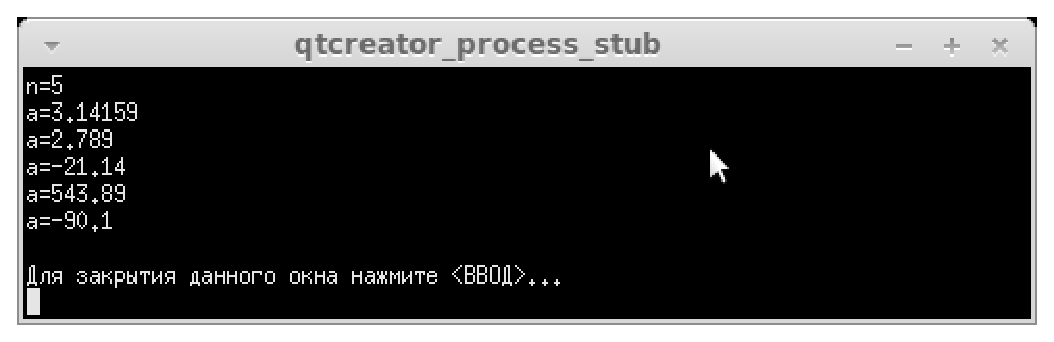
\includegraphics[width=0.8\textwidth]{img/ris_7_1}
\caption{Процесс работы программы к задаче \ref{ch07:prg0}. Ввод исходных данных.}
\label{ch07:refDrawing0}
\end{center}
\end{figure}
\begin{figure}[htb]
\begin{center}
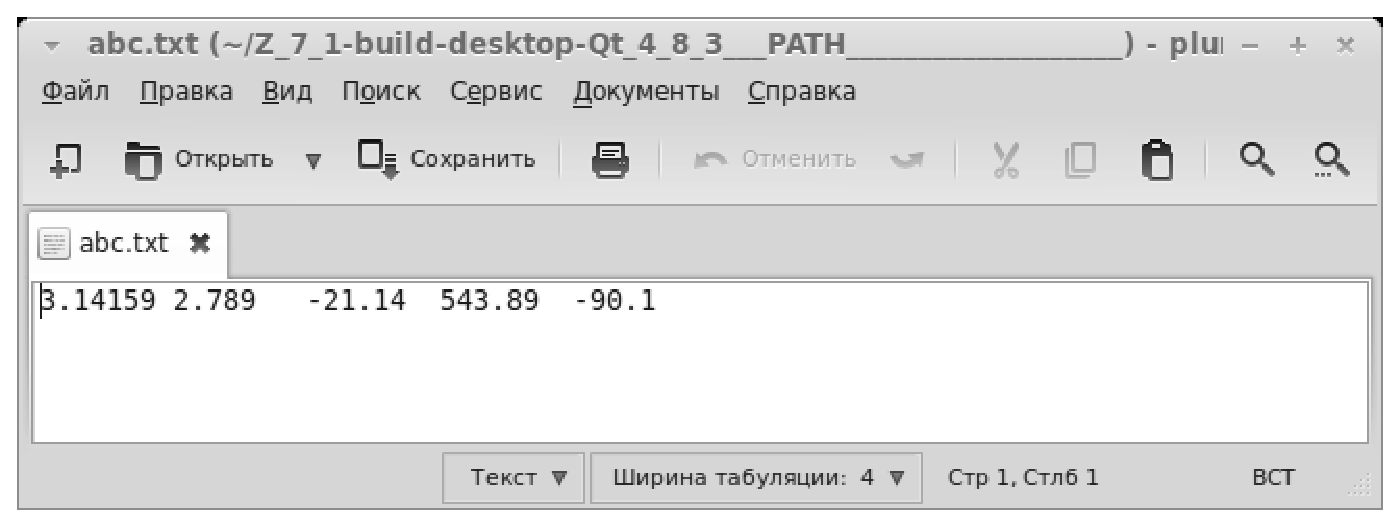
\includegraphics[width=0.8\textwidth]{img/ris_7_2}
\caption{Текстовый файл \Sys{abc.txt}, созданный программой к задаче~\ref{ch07:prg0}.}
\label{ch07:refDrawing1}
\end{center}
\end{figure}

\subsection[Чтение информации из текстового файла]{Чтение информации из текстового файла}\label{ch07:2.2}

Для того, чтобы \emph{прочитать информацию из текстового файла},
необходимо описать переменную типа \Sys{ifstream}. После этого файл необходимо открыть для чтения с
помощью оператора \Sys{open}. Если переменную назвать \Sys{F}, то первые два оператора будут
такими:

\Sys{ifstream F;}

\Sys{F.open(\symbol{`\"}abc.txt\symbol{`\"}, ios::in);}\footnote{Указание режима \Sys{ios::in} можно, конечно, опустить,
ведь для потока \Sys{ifstream} значение \Sys{ios::in} является значением по умолчанию, тогда 
оператор open можно будет записать так \lstinline!F.open("abc.txt");!}

После открытия файла в \emph{режиме чтения}, из него можно считывать информацию точно так же, как и с
клавиатуры, только вместо стандартного устройства ввода \Sys{cin} необходимо указать
\emph{имя потока}, из которого будет происходить чтение данных.

Например, для чтения из потока \Sys{F} в переменную \Sys{a} оператор ввода будет иметь вид:

\Sys{F{>}{>}a;}

Для последовательного ввода из потока \Sys{G} в переменные \Sys{b}, \Sys{с} и
\Sys{d} оператор ввода станет таким:

\Sys{G{>}{>}b{>}{>}c{>}{>}d;}

Два числа в текстовом файле считаются разделёнными, если между ними есть хотя бы один из символов: пробел, табуляция,
символ конца строки.

Хорошо, если программисту заранее известно, сколько и каких значений хранится в текстовом файле. Однако часто просто
известен тип значений, хранящихся в файле, при этом количество значений в файле может быть различным. При решении
подобной проблемы необходимо считывать значения из файла по одному, а перед каждым считыванием проверять, достигнут ли
конец файла. Для проверки, достигнут или нет \emph{конец файла}, служит функция 

\Sys{F.eof();}

Здесь \Sys{F} --- имя потока, функция возвращает логическое значение: \Sys{true} --- если
достигнут конец файла, если не достигнут функция возвращает значение \Sys{false}.

Следовательно, цикл для чтения содержимого всего файла можно записать так.
\begin{lstlisting}
while (!F.eof()) //`Организован цикл, условием окончания цикла`
//`является достижение конца файла, в этом случае \Sys{F.eof()} вернёт \Sys{true}.`
{
  F>>a;	//`Чтение очередного значения из потока \Sys{F} в переменную \Sys{a}.`
  `...`
  `<обработка значения переменной \Sys{a}>`
}
\end{lstlisting}

Рассмотрим следующую задачу.

\prg{В текстовом файле \emph{abc.txt} хранятся вещественные числа (рис.~\ref{ch07:refDrawing1}), 
вывести их на экран и вычислить их количество.}{ch07:prg1}

Текст программы с комментариями приведён ниже.
\begin{lstlisting}
#include <iostream>
#include <fstream>
using namespace std;
int main()
{
  ifstream f; //`Поток для чтения.`
  float a; int n=0;
  f.open("abc.txt"); //`Открываем файл в режиме чтения.`
  if (f) //`Если открытие файла	прошло корректно, то`
  {
    while (!f.eof()) //`Организован цикл, выполнение цикла`
    //`прервётся, когда будет достигнут конца файла.`
    {
      f>>a; //`Чтение очередного значения из потока \Sys{f} в переменную \Sys{a}.`
      cout<<a<<"\t"; //`Вывод значения переменной \Sys{a}` 
      n++;  //`Увеличение количества считанных чисел.`
    }
    f.close(); //`Закрытие потока.`
    cout<<"n="<<n<<endl; //`Вывод на экран количества чисел.`
  }
  else cout<<"`\Sys{Файл не найден}`"<<endl; //`Если открытие файла прошло некорректно, то`
  //`вывод сообщения, об отсутствии такого файла.`
  return 0;
}
\end{lstlisting}

Результат работы программы к задаче~\ref{ch07:prg1}:
\begin{verbatim}
3.14159 2.789 -21.14 543.89 -90.1  n=5
\end{verbatim}

Программа работает корректно, если текстовый файл \Sys{abc.txt} был создан с помощью 
программы к задаче~\ref{ch07:prg0}. Предположим, что файл создавался в текстовом редакторе, 
и пользователь ввёл после последней цифры символ пробела, табуляции или перехода на новую строку. 
Тогда результат будет таким:
\begin{verbatim}
3.14159 2.789 -21.14 543.89 -90.1 -90.1  n= 6
\end{verbatim}

Происходит это потому, что после чтения последней цифры из потока конец файла не достигнут, оператор 
цикла выполняется ещё один раз, значение переменной $n$ увеличивается на единицу, а так как значение 
переменной $a$ не изменилось, то выводится повторно. Один из способов решения данной проблемы может быть таким:
\begin{lstlisting}
while (!f.eof())
{
  f>>a;
  if (!f.eof()) //`Проверяем, достигнут ли конец файла, если нет --- печатаем значение a`
  {
    cout<<a<<"\t";
    n++;
  }
}
\end{lstlisting}

Если количество вещественных чисел, записанных в файл, известно заранее, то текст программы можно переписать следующим
образом:

\begin{lstlisting}
#include <iostream>
#include <fstream>
using namespace std;
int main()
{
  ifstream f;
  float a; int i,n=5;
  f.open("abc.txt");
  if (f)
  {
    for (i=1;i<=n;f>>a,cout<<a<<"\t",i++);
      f.close();
  }
  else cout<<"`\Sys{Файл не найден}`"<<endl;
  return 0;
}
\end{lstlisting}

Существует возможность открывать файл с данными таким образом, чтобы в него можно было \emph{дописывать
информацию}. Рассмотрим эту возможность на примере решения следующей задачи.

\prg{В файле \emph{abc.txt} (рис.~\ref{ch07:refDrawing1})
хранится массив вещественных чисел, дописать в файл этот же массив, упорядочив его по возрастанию.}{ch07:prg2}

Алгоритм решения задачи очень простой. Считываем в массив данные из текстового файла, упорядочиваем массив, дописываем
его в этот же файл.

Для чтения данных из файла описываем поток \Sys{ifstream}, открываем его в режиме чтения и последовательно,
пока не достигнем конца файла, считываем все элементы в массив. Сортировку проведём методом пузырька. Обратите
внимание, что поток нужно открыть так, чтобы была возможность дописать в конец файла упорядоченный массив.

Текст программы с комментариями приведён ниже. %Результаты работы программы показаны на рис. \ref{ch07:ref2a}.
\begin{lstlisting}
#include <iostream>
#include <fstream>
using namespace std;
int main()
{
  ifstream f; //`Поток для чтения.`
  ofstream g; //`Поток для записи.`
  float *a,b;
  a=new float[100];
  int i,j,n=0;
  f.open("abc.txt",ios::in); //`Открываем файл в режиме чтения.`
  if (f)	
  {
    while (!f.eof())
    {
      f>>a[n];
      n++;
    }
    //`Сортировка массива.`
    for(i=0;i<n-1;i++)
      for(j=0;j<n-i-1;j++)
        if (a[j]>a[j+1])
        {
          b=a[j];
          a[j]=a[j+1];
          a[j+1]=b;
        }
    f.close(); //`Закрываем поток для чтения.`
    g.open("abc.txt",ios::app); //`Открываем поток для того, чтобы дописать данные.`
    g<<"\n"; //`Запись в файл символа конца строки` 
    for(i=0;i<n;i++) //`Запись в файл`
      if (i<n-1) g<<a[i]<< "\t" ;	//`элемента массива и символа табуляции.`
      else  g<<a[i];  //`Запись последнего элемента массива`
    g.close(); //`Закрытие файла.`
  }
  else cout<<"`\Sys{Файл не найден}`"<<endl;
  delete [] a;
  return 0;
}
\end{lstlisting}

Содержимое файла \Sys{abc.txt} после запуска программы к задаче~\ref{ch07:prg2}
\begin{verbatim}
3.14159 2.798 -21.14 543.89 -90.1
-90.1 -21.14 2.798 3.14159 543.89
\end{verbatim}


\section[Обработка двоичных файлов]{Обработка двоичных файлов}
Если в файле хранятся только числа или данные определённой структуры, то для хранения таких значений удобно пользоваться
двоичными файлами. В \index{Файл!двоичный}\emph{двоичных файлах} информация считывается и записывается в
виде блоков определённого размера, в них могут храниться данные любого вида и структуры.

Порядок работы с двоичными и текстовыми файлами аналогичен. Для того, чтобы
\index{Файл!запись}\emph{записать данные в двоичный файл}, необходимо:

\begin{enumerate}
\item Описать файловую переменную с помощью оператора
\Sys{FILE *filename;}
Здесь \Sys{filename} --- имя переменной, где будет храниться указатель на файл.
\item Открыть файл с помощью функции \Sys{fopen}.
\item Записать информацию в файл с помощью функции \Sys{fwrite}.
\item Закрыть файл с помощью функции \Sys{fclose}.
\end{enumerate}
Для того, чтобы \index{Файл!чтение}\emph{считывать данные из двоичного файла}, необходимо:

\begin{enumerate}
\item Описать переменную типа \Sys{FILE *}.
\item Открыть файл с помощью функции \Sys{fopen}.
\item Считать необходимую информацию из файла с помощью функции \Sys{fread}, при считывании информации
следить за тем, достигнут ли конец файла.
\item Закрыть файл с помощью функции \Sys{fclose}.
\end{enumerate}
Рассмотрим основные функции, необходимые для работы с двоичными файлами.

Для \index{Файл!открыть}\emph{открытия файла} предназначена функция:

\Sys{FILE *fopen(const *filename, const char *mode);}
где, \Sys{filename} --- строка, в которой хранится полное имя открываемого файла, \Sys{mode} ---
строка, которая определяет режим работы с файлом; возможны следующие значения:
\begin{itemize}
\item[] «\Sys{rb}» --- открыть двоичный файл в режиме чтения;
\item[] «\Sys{wb}» --- создать двоичный файл для записи, если файл существует, то его содержимое очищается.
\item[] «\Sys{ab}» --- создать или открыть двоичный файл для добавления информации в конец файла;
\item[] «\Sys{rb+}» --- открыть существующий двоичный файл в режиме чтения и записи;
\item[] «\Sys{wb+}» --- открыть двоичный файл в режиме чтения и записи, существующий файл очищается;
\item[] «\Sys{ab+}» --- двоичный файл открывается или создаётся для исправления существующей информации и
добавления новой в конец файла.
\end{itemize}
Функция \Sys{fopen} возвращает в файловой переменной \Sys{NULL} в случае неудачного открытия файла.

После открытия файла, в указателе содержится адрес 0-го байта файла. По мере чтения или записи значение указателя
смещается на считанное (записанное) количество байт. Текущее значение указателя --- номер байта, начиная с которого будет
происходить операция чтения или записи.

Для \index{Файл!закрыть}\emph{закрытия файла} предназначена функция

\Sys{int fclose(FILE *filename);}

Она возвращает 0 при успешном закрытии файла и \Sys{NULL} в противном случае.

Для \index{Файл!удаление}\emph{удаления файлов} существует функция

\Sys{int remove(const char *filename);}

Эта функция удаляет с диска файл с именем \Sys{filename}. Удаляемый файл должен быть закрыт. Функция
возвращает ненулевое значение, если файл не удалось удалить.

Для \index{Файл!переименование}\emph{переименования файлов} предназначена функция

\Sys{int rename(const char *oldfilename, const char *newfilename);}

здесь первый параметр --- старое имя файла, второй --- новое. Возвращает 0 при удачном завершении программы.

\index{Файл!чтение}\emph{Чтение из двоичного файла} осуществляется с помощью функции

\Sys{fread (void *ptr, size, n, FILE *filename)}

Эта функция считывает из файла \Sys{filename} в массив \Sys{ptr}  \Sys{n}
элементов размера \Sys{size}. Функция возвращает количество считанных элементов. После чтения из файла
указатель файла смещается на \Sys{n*size} байт.

\index{Файл!запись}\emph{Запись в двоичный файл} осуществляется с помощью функции

\Sys{fwrite (const void *ptr, size, n, FILE *filename);}

Функция записывает в файл \Sys{filename} из массива \Sys{ptr} \Sys{n} элементов
размера \Sys{size}. Функция возвращает количество записанных элементов. После записи информации в файл,
указатель файла смещается на \Sys{n*size} байт.

Для контроля достижения конца файла есть функция

\Sys{int feof(FILE * filename);}

Она возвращает ненулевое значение, если достигнут конец файла.

Рассмотрим использование двоичных файлов на примере решения двух стандартных задач.

\prg{Создать двоичный файл \emph{abc.dat}, куда
записать целое число \emph{n} и \emph{n} вещественных чисел.}{ch07:prg3}
\begin{lstlisting}
#include <iostream>
#include <fstream>
using namespace std;
int main()
{
  FILE *f; //`Описание файловой переменной.`
  int i, n; double a;
  f=fopen("abc.dat","wb"); //`Создание двоичного файла в режиме записи.`
  cout<<"n="; cin>>n; //`Ввод числа \Sys{n}.`
  fwrite(&n,sizeof(int),1,f); //`Запись числа в двоичный файл.`
  for(i=0;i<n;i++) //`Цикл для ввода \Sys{n} вещественных чисел.`
  {
    cout<<"a="; cin>>a; //`Ввод очередного вещественного числа.`
    fwrite(&a,sizeof(double),1,f); //`Запись числа в двоичный файл.`
  }
  fclose(f); //`Закрыть файл.`
  return 0;
}
\end{lstlisting}

\prg{Вывести на экран содержимое созданного в задаче \ref{ch07:prg3} двоичного файла
\Sys{abc.dat}.}{ch07:prg4}
\begin{lstlisting}
#include <iostream>
#include <fstream>
using namespace std;
int main()
{
  FILE *f; //`Описание файловой переменной.`
  int i,n; double *a;
  f=fopen("abc.dat","rb"); //`Открыть существующий двоичный файл в режиме чтения.`
  fread(&n,sizeof(int),1,f);//`Читать из файла целое число в переменную \Sys{n}.`
  cout<<"n="<<n<<"\n";//`Вывод \Sys{n} на экран.`
  a=new double[n]; //`Выделение памяти для массива из \Sys{n} чисел.`
  fread(a,sizeof(double),n,f);//`Чтение \Sys{n} вещественных чисел из файла в массив \Sys{a}.`
  for(i=0;i<n;cout<<a[i]<<"\t",i++); //`Вывод массива на экран.`
    cout<<endl;
  fclose(f); //`Закрыть файл.`
  return 0;
}
\end{lstlisting}

\emph{Двоичный файл }--- последовательная структура данных, после открытия файла доступен первый байт. Можно
последовательно считывать из файла или записывать их в него. Допустим, необходимо считать пятнадцатое, а затем первое
число, хранящееся в файле. С помощью \index{Файл!последовательный доступ}\emph{последовательного доступа}
это можно сделать следующим образом.
\begin{lstlisting}
FILE *f; 
int i,n; double a;
f=fopen("file.dat","rb");
for(i=0;i<15;fread(&a,sizeof(double),1,f),i++);
fclose(f);
f=fopen("file.dat","rb");
fread(&a,sizeof(double),1,f);
fclose(f);
\end{lstlisting}

Как видно, такое чтение чисел из файла, а затем повторное открытие файла --- не самый удачный способ. Гораздо удобнее
использовать \emph{функцию перемещения указателя файла} к заданному байту:

\Sys{int fseek(FILE *F, long int offset, int origin);}

Функция устанавливает указатель текущей позиции файла \Sys{F}, в соответствии со значениями начала отсчёта
\Sys{origin} и смешения \Sys{offset}. Параметр \Sys{offset} равен количеству
байтов, на которые будет смещён указатель файла относительно начала отсчёта, заданного параметром
\Sys{origin}. Если значение \Sys{offset} положительно, то указатель файла смещается вперёд,
если отрицательно --- назад. Параметр \Sys{origin} должен принимать одно из следующих значений, 
определённых в заголовке \Sys{stdio.h:}
\begin{itemize}
\item[] \Sys{SEEK\_SET} --- отсчёт смещения \Sys{offset} вести с начала файла;
\item[] \Sys{SEEK\_CUR} --- отсчёт смещения \Sys{offset} вести с текущей позиции файла;
\item[] \Sys{SEEK\_END} --- отсчёт смещения \Sys{offset} вести с конца файла.
\end{itemize}
Функция возвращает нулевое значение при успешном выполнении операции и ненулевое, если возник сбой при выполнении
смещения.

Функция \Sys{fseek} фактически реализует прямой доступ к любому значению в файле. Необходимо только знать
месторасположение (номер байта) значения в файле. Рассмотрим использование прямого доступа в двоичных файлах на примере
решения следующей задачи.

\prg{В созданном в задаче~\ref{ch07:prg3} двоичном файле \emph{abc.dat}
поменять местами наибольшее и наименьшее из вещественных чисел.}{ch07:prg5}

Алгоритм решения задачи состоит из следующих этапов:

\begin{enumerate}
\item Чтение вещественных чисел из файла в массив \Sys{a}.
\item Поиск в массиве \Sys{a} максимального (\Sys{max}) и минимального
(\Sys{min}) значения и их номеров (\Sys{imax}, \Sys{imin}).
\item Перемещение указателя файла к максимальному значению и запись \Sys{min}.
\item Перемещение указателя файла к минимальному значению и запись \Sys{max}.
\end{enumerate}
Ниже приведён текст программы решения задачи с комментариями.
\begin{lstlisting}
#include <iostream>
#include <fstream>
using namespace std;
int main()
{
  FILE *f; //`Описание файловой переменной.` 
  int i,n,imax, imin;
  double *a, max,min;
  f=fopen("abc.dat","rb+");//`Открыть файл в режиме чтения и записи.`
  fread(&n,sizeof(int),1,f);//`Считать из файла в переменную n количество элементов в файле.`
  a=new double[n];//`Выделить память для хранения вещественных чисел,`
                  //`эти числа будут хранится в массиве a.`
  fread(a,sizeof(double),n,f);//`Считать из файла в массив a вещественные числа.`
  //`Поиск максимального, минимального элемента в массиве a, и их индексов.`
  for(imax=imin=0, max=min=a[0],i=1;i<n;i++) 
  {
    if (a[i]>max) 
    {
      max=a[i];
      imax=i;
    }
    if (a[i]<min)
    {
      min=a[i];
      imin=i;
    }
  }
  //`Перемещение указателя к максимальному элементу.`
  fseek(f,sizeof(int)+imax*sizeof(double),SEEK_SET);
  //`Запись min вместо максимального элемента файла.`
  fwrite(&min,sizeof(double),1,f);
  //`Перемещение указателя к минимальному элементу.`
  fseek(f,sizeof(int)+imin*sizeof(double),SEEK_SET);
  //`Запись max вместо минимального элемента файла.`
  fwrite(&max,sizeof(double),1,f);
  //`Закрытие файла.`
  fclose(f);
  //`Освобождение памяти, выделенной под массив a.`
  delete []a;
  return 0;
}
\end{lstlisting}

\section[Функции fscanf() и fprintf()]{Функции fscanf() и fprintf()}
Чтение и запись данных в файл можно выполнять с помощью функций \Sys{fscanf()} и
\Sys{fprintf()}. Эти функции подобны функциям \Sys{scanf()} и
\Sys{printf()}, описанным в п.~\ref{ch02:9}, за тем исключением, что работают не с клавиатурой и
экраном, а с файлами. Функции имеют следующие прототипы.

\emph{Функция чтения}

\Sys{fscanf(указатель на файл, строка форматов, адреса переменных);}

\emph{Функция записи}

\Sys{fprintf(указатель на файл,строка форматов, список переменных);}

Далее приведён фрагмент программного кода, который демонстрирует пример записи информации в файл
\Sys{my.txt}.
\begin{lstlisting}
char fio[30]="`\Sys{Махарадзе В.}`";
int a=5, b=5, c=4;
float s= (float) (a+b+c)/3;
FILE *f;
f=fopen("my.txt","w");
fprintf(f,"`\Sys{Оценки студента}` %s \n", fio);
fprintf(f,"`\Sys{математика}` %d, `\Sys{физика}` %d, `\Sys{химия}` %d \n", a,b,c);
fprintf(f,"`\Sys{Средний балл}` = %.2f \n", s);
fprintf(f,"\n");
fclose(f);
\end{lstlisting}

В результате будет сформирован текстовый файл:
\begin{verbatim}
Оценки студента Махарадзе В.
математика 5, физика 5, химия 4
Средний балл = 4.67
\end{verbatim}

Рассмотрим пример чтения данных из файла. Пусть в файле \Sys{test.txt} хранится информация:
\begin{verbatim}
1 Иванов Пётр  170 78.1
2 Петров Иван  180 89.6
3 Карпов Борис 167 56.7
\end{verbatim}

Тогда с помощью следующих команд можно считать информацию из файла и вывести её на экран.
\begin{lstlisting}
int i,nom;
float Ves;
int Rost;
char fio[15],name[15];
FILE *f;	
f=fopen("test.txt","r");
for (i=0;i<3;i++)
{
  //`Чтение из файла`
  fscanf(f,"%d%s%s%d%f \n",&nom, &fio,&name,&Rost,&Ves);
  //`Вывод на экран`
  printf("%d %s %s %d %.2f \n",nom,fio,name,Rost,Ves);
}
fclose(f);
\end{lstlisting}
